\documentclass[qualitaetssicherung.tex]{subfiles}

\begin{document}

\section{Webbrowser - Zeichnen von SVG-Grafiken}
	\subsection{Einleitung}
	Bei der Einparkhilfe verwenden wir SVG-Grafiken, um den Pfad des Autos zu zeichnen. Um es gut abschätzen zu können, wie schnell die verschiedene Webbrowser SVG-Grafiken zeichnen können ist es Sinnvoll eine einfache HTML-Datei zu schreiben, die sich immer wieder neu lädt. Die Frage ist, wie lange dauert es, bis alles gezeichnet wird?
	\subsection{Ablauf}
	\begin{itemize}
	\item Da wir nicht genau wissen, wie gut die Darstellung intern parallelisiert ist, weisen wir Firefox einen einzigen Prozessorkern zu (64-bit, 2.5 GHz). Wir schalten alle Puffern aus, damit es immer wieder neu geladen und gezeichnet wird. Windows 7 puffert jedoch das Bild im Hintergrund, das heißt, dass wir nicht auf Festplattenzugriffe achten müssen.
	\item Wir öffnen eine HTML-Datei, die lediglich ein SVG Bild enthält und stellen sicher, dass es immer wieder neu geladen wird. Zum Beispiel, wenn wir die Zeile <META HTTP-EQUIV="refresh" CONTENT="1"> in die HTML-Datei einfügen, dann wird sie alle Sekunden neu geladen.
	\item Wir öffnen mehr und mehr Tabs und beobachten, wie stark der Prozessorkern belastet wird (Abb. ~\ref{firefox_svg}).
	\item In unserem Fall können wir 20 Tabs öffnen und die Belastung beträgt 61\%. Dies bedeutet, dass es 0.61 x 1000 ms / 20 = 30.5 ms dauert das Bild in Firefox zu zeichnen.
	\item Hinweis: Wir haben nur bewiesen, dass Firefox maximal 31 ms braucht um das Bild zu zeichnen, es ist möglich, dass der Wert weniger ist.
	
	\begin{figure}[H]
    \textbf{Firefox mit 20 SVG Tabs}\par\medskip
    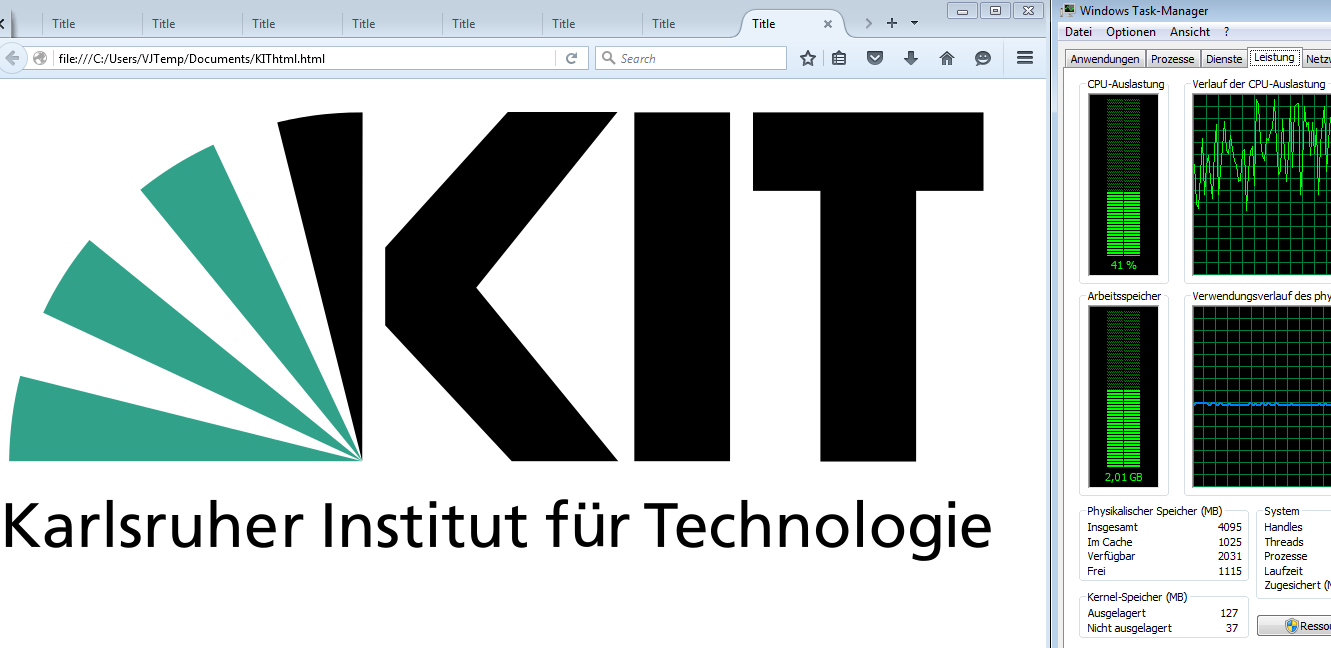
\includegraphics[width=0.99\textwidth]{Images/firefox-svg.png}
    \caption{Durchschnittliche Auslastung des CPU-Kerns: 61\%}
		\label{firefox_svg}
	\end{figure}
	\end{itemize}
	
\end{document}